% Scatter plot: E1 cost vs deterministic exit criteria
% Usage: % Scatter plot: E1 cost vs deterministic exit criteria
% Usage: % Scatter plot: E1 cost vs deterministic exit criteria
% Usage: % Scatter plot: E1 cost vs deterministic exit criteria
% Usage: \input{generated/scatter-cost-performance.tex}
%
% Deterministic criteria (10 total):
%   P1-P5 = checkmark, Q1 = match, Q2 = 42/42, Q5 = 0, Q6 = 0, Q7 = 0
%
% Data source: Tab. cross-run (kap04), costs from E1 estimates

\begin{figure}[H]
\centering
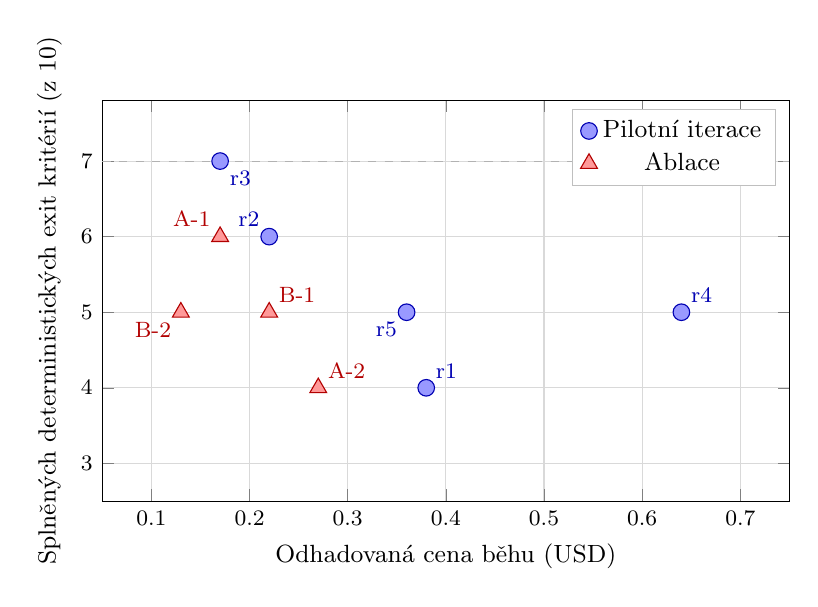
\begin{tikzpicture}
\begin{axis}[
    width=0.85\textwidth,
    height=0.55\textwidth,
    xlabel={Odhadovaná cena běhu (USD)},
    ylabel={Splněných deterministických exit kritérií (z~10)},
    xmin=0.05, xmax=0.75,
    ymin=2.5, ymax=7.8,
    ytick={3,4,5,6,7},
    grid=major,
    grid style={gray!30},
    legend style={
        at={(0.98,0.98)},
        anchor=north east,
        font=\small,
        draw=gray!50,
    },
    every axis label/.style={font=\small},
    tick label style={font=\footnotesize},
    clip=false,
]

% Pilot runs (circle markers, blue)
\addplot[
    only marks,
    mark=*,
    mark size=3pt,
    color=blue!70!black,
    fill=blue!40,
] coordinates {
    (0.38, 4)   % r1
    (0.22, 6)   % r2
    (0.17, 7)   % r3
    (0.64, 5)   % r4
    (0.36, 5)   % r5
};
\addlegendentry{Pilotní iterace}

% Ablation runs (triangle markers, red/orange)
\addplot[
    only marks,
    mark=triangle*,
    mark size=3.5pt,
    color=red!70!black,
    fill=red!40,
] coordinates {
    (0.17, 6)   % A-1
    (0.27, 4)   % A-2
    (0.22, 5)   % B-1
    (0.13, 5)   % B-2
};
\addlegendentry{Ablace}

% Labels for pilot runs
\node[above right, font=\footnotesize, blue!70!black]
    at (axis cs:0.38, 4) {r1};
\node[above left, font=\footnotesize, blue!70!black]
    at (axis cs:0.22, 6) {r2};
\node[below right, font=\footnotesize, blue!70!black]
    at (axis cs:0.17, 7) {r3};
\node[above right, font=\footnotesize, blue!70!black]
    at (axis cs:0.64, 5) {r4};
\node[below left, font=\footnotesize, blue!70!black]
    at (axis cs:0.36, 5) {r5};

% Labels for ablation runs
\node[above left, font=\footnotesize, red!70!black]
    at (axis cs:0.17, 6) {A-1};
\node[above right, font=\footnotesize, red!70!black]
    at (axis cs:0.27, 4) {A-2};
\node[above right, font=\footnotesize, red!70!black]
    at (axis cs:0.22, 5) {B-1};
\node[below left, font=\footnotesize, red!70!black]
    at (axis cs:0.13, 5) {B-2};

% Reference line at r3 performance level
\draw[dashed, gray!60, thin]
    (axis cs:0.05, 7) -- (axis cs:0.75, 7);

\end{axis}
\end{tikzpicture}
\caption[Cena běhu vs.\ počet splněných deterministických exit kritérií]{%
    Vztah mezi odhadovanou cenou běhu (E1) a~počtem splněných
    deterministických exit kritérií (P1--P5, Q1, Q2${=}$42/42,
    Q5${=}$0, Q6${=}$0, Q7${=}$0). Běh~r3 dosáhl nejvyšší hodnoty
    7/10 při nejnižší ceně z~pilotních iterací. Ablační běhy
    (trojúhelníky) se pohybují v~rozmezí 4--6 splněných kritérií.}
\label{fig:scatter-cost-perf}
\end{figure}

%
% Deterministic criteria (10 total):
%   P1-P5 = checkmark, Q1 = match, Q2 = 42/42, Q5 = 0, Q6 = 0, Q7 = 0
%
% Data source: Tab. cross-run (kap04), costs from E1 estimates

\begin{figure}[H]
\centering
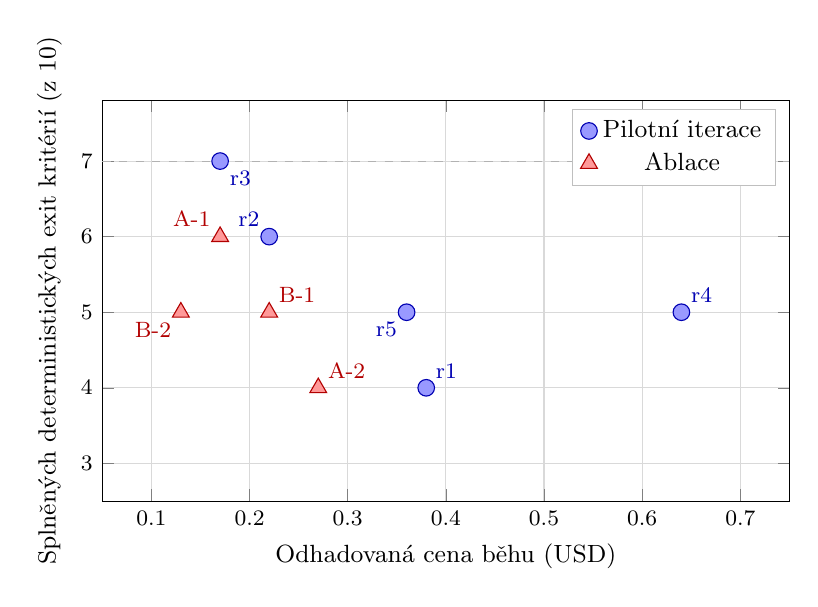
\begin{tikzpicture}
\begin{axis}[
    width=0.85\textwidth,
    height=0.55\textwidth,
    xlabel={Odhadovaná cena běhu (USD)},
    ylabel={Splněných deterministických exit kritérií (z~10)},
    xmin=0.05, xmax=0.75,
    ymin=2.5, ymax=7.8,
    ytick={3,4,5,6,7},
    grid=major,
    grid style={gray!30},
    legend style={
        at={(0.98,0.98)},
        anchor=north east,
        font=\small,
        draw=gray!50,
    },
    every axis label/.style={font=\small},
    tick label style={font=\footnotesize},
    clip=false,
]

% Pilot runs (circle markers, blue)
\addplot[
    only marks,
    mark=*,
    mark size=3pt,
    color=blue!70!black,
    fill=blue!40,
] coordinates {
    (0.38, 4)   % r1
    (0.22, 6)   % r2
    (0.17, 7)   % r3
    (0.64, 5)   % r4
    (0.36, 5)   % r5
};
\addlegendentry{Pilotní iterace}

% Ablation runs (triangle markers, red/orange)
\addplot[
    only marks,
    mark=triangle*,
    mark size=3.5pt,
    color=red!70!black,
    fill=red!40,
] coordinates {
    (0.17, 6)   % A-1
    (0.27, 4)   % A-2
    (0.22, 5)   % B-1
    (0.13, 5)   % B-2
};
\addlegendentry{Ablace}

% Labels for pilot runs
\node[above right, font=\footnotesize, blue!70!black]
    at (axis cs:0.38, 4) {r1};
\node[above left, font=\footnotesize, blue!70!black]
    at (axis cs:0.22, 6) {r2};
\node[below right, font=\footnotesize, blue!70!black]
    at (axis cs:0.17, 7) {r3};
\node[above right, font=\footnotesize, blue!70!black]
    at (axis cs:0.64, 5) {r4};
\node[below left, font=\footnotesize, blue!70!black]
    at (axis cs:0.36, 5) {r5};

% Labels for ablation runs
\node[above left, font=\footnotesize, red!70!black]
    at (axis cs:0.17, 6) {A-1};
\node[above right, font=\footnotesize, red!70!black]
    at (axis cs:0.27, 4) {A-2};
\node[above right, font=\footnotesize, red!70!black]
    at (axis cs:0.22, 5) {B-1};
\node[below left, font=\footnotesize, red!70!black]
    at (axis cs:0.13, 5) {B-2};

% Reference line at r3 performance level
\draw[dashed, gray!60, thin]
    (axis cs:0.05, 7) -- (axis cs:0.75, 7);

\end{axis}
\end{tikzpicture}
\caption[Cena běhu vs.\ počet splněných deterministických exit kritérií]{%
    Vztah mezi odhadovanou cenou běhu (E1) a~počtem splněných
    deterministických exit kritérií (P1--P5, Q1, Q2${=}$42/42,
    Q5${=}$0, Q6${=}$0, Q7${=}$0). Běh~r3 dosáhl nejvyšší hodnoty
    7/10 při nejnižší ceně z~pilotních iterací. Ablační běhy
    (trojúhelníky) se pohybují v~rozmezí 4--6 splněných kritérií.}
\label{fig:scatter-cost-perf}
\end{figure}

%
% Deterministic criteria (10 total):
%   P1-P5 = checkmark, Q1 = match, Q2 = 42/42, Q5 = 0, Q6 = 0, Q7 = 0
%
% Data source: Tab. cross-run (kap04), costs from E1 estimates

\begin{figure}[H]
\centering
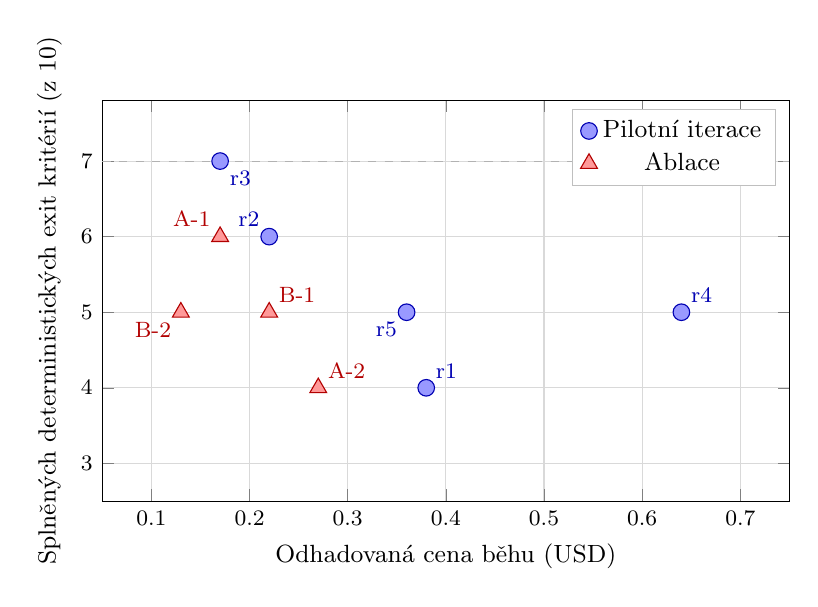
\begin{tikzpicture}
\begin{axis}[
    width=0.85\textwidth,
    height=0.55\textwidth,
    xlabel={Odhadovaná cena běhu (USD)},
    ylabel={Splněných deterministických exit kritérií (z~10)},
    xmin=0.05, xmax=0.75,
    ymin=2.5, ymax=7.8,
    ytick={3,4,5,6,7},
    grid=major,
    grid style={gray!30},
    legend style={
        at={(0.98,0.98)},
        anchor=north east,
        font=\small,
        draw=gray!50,
    },
    every axis label/.style={font=\small},
    tick label style={font=\footnotesize},
    clip=false,
]

% Pilot runs (circle markers, blue)
\addplot[
    only marks,
    mark=*,
    mark size=3pt,
    color=blue!70!black,
    fill=blue!40,
] coordinates {
    (0.38, 4)   % r1
    (0.22, 6)   % r2
    (0.17, 7)   % r3
    (0.64, 5)   % r4
    (0.36, 5)   % r5
};
\addlegendentry{Pilotní iterace}

% Ablation runs (triangle markers, red/orange)
\addplot[
    only marks,
    mark=triangle*,
    mark size=3.5pt,
    color=red!70!black,
    fill=red!40,
] coordinates {
    (0.17, 6)   % A-1
    (0.27, 4)   % A-2
    (0.22, 5)   % B-1
    (0.13, 5)   % B-2
};
\addlegendentry{Ablace}

% Labels for pilot runs
\node[above right, font=\footnotesize, blue!70!black]
    at (axis cs:0.38, 4) {r1};
\node[above left, font=\footnotesize, blue!70!black]
    at (axis cs:0.22, 6) {r2};
\node[below right, font=\footnotesize, blue!70!black]
    at (axis cs:0.17, 7) {r3};
\node[above right, font=\footnotesize, blue!70!black]
    at (axis cs:0.64, 5) {r4};
\node[below left, font=\footnotesize, blue!70!black]
    at (axis cs:0.36, 5) {r5};

% Labels for ablation runs
\node[above left, font=\footnotesize, red!70!black]
    at (axis cs:0.17, 6) {A-1};
\node[above right, font=\footnotesize, red!70!black]
    at (axis cs:0.27, 4) {A-2};
\node[above right, font=\footnotesize, red!70!black]
    at (axis cs:0.22, 5) {B-1};
\node[below left, font=\footnotesize, red!70!black]
    at (axis cs:0.13, 5) {B-2};

% Reference line at r3 performance level
\draw[dashed, gray!60, thin]
    (axis cs:0.05, 7) -- (axis cs:0.75, 7);

\end{axis}
\end{tikzpicture}
\caption[Cena běhu vs.\ počet splněných deterministických exit kritérií]{%
    Vztah mezi odhadovanou cenou běhu (E1) a~počtem splněných
    deterministických exit kritérií (P1--P5, Q1, Q2${=}$42/42,
    Q5${=}$0, Q6${=}$0, Q7${=}$0). Běh~r3 dosáhl nejvyšší hodnoty
    7/10 při nejnižší ceně z~pilotních iterací. Ablační běhy
    (trojúhelníky) se pohybují v~rozmezí 4--6 splněných kritérií.}
\label{fig:scatter-cost-perf}
\end{figure}

%
% Deterministic criteria (10 total):
%   P1-P5 = checkmark, Q1 = match, Q2 = 42/42, Q5 = 0, Q6 = 0, Q7 = 0
%
% Data source: Tab. cross-run (kap04), costs from E1 estimates

\begin{figure}[H]
\centering
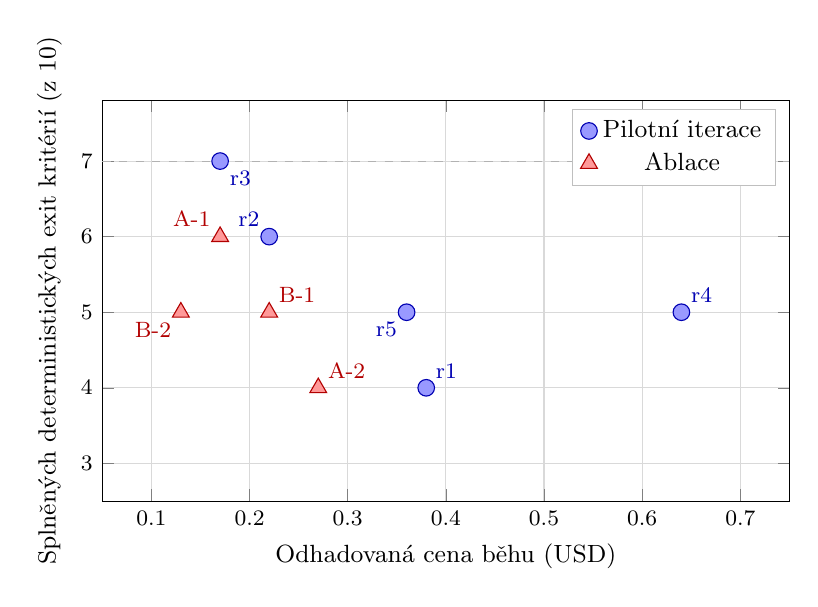
\begin{tikzpicture}
\begin{axis}[
    width=0.85\textwidth,
    height=0.55\textwidth,
    xlabel={Odhadovaná cena běhu (USD)},
    ylabel={Splněných deterministických exit kritérií (z~10)},
    xmin=0.05, xmax=0.75,
    ymin=2.5, ymax=7.8,
    ytick={3,4,5,6,7},
    grid=major,
    grid style={gray!30},
    legend style={
        at={(0.98,0.98)},
        anchor=north east,
        font=\small,
        draw=gray!50,
    },
    every axis label/.style={font=\small},
    tick label style={font=\footnotesize},
    clip=false,
]

% Pilot runs (circle markers, blue)
\addplot[
    only marks,
    mark=*,
    mark size=3pt,
    color=blue!70!black,
    fill=blue!40,
] coordinates {
    (0.38, 4)   % r1
    (0.22, 6)   % r2
    (0.17, 7)   % r3
    (0.64, 5)   % r4
    (0.36, 5)   % r5
};
\addlegendentry{Pilotní iterace}

% Ablation runs (triangle markers, red/orange)
\addplot[
    only marks,
    mark=triangle*,
    mark size=3.5pt,
    color=red!70!black,
    fill=red!40,
] coordinates {
    (0.17, 6)   % A-1
    (0.27, 4)   % A-2
    (0.22, 5)   % B-1
    (0.13, 5)   % B-2
};
\addlegendentry{Ablace}

% Labels for pilot runs
\node[above right, font=\footnotesize, blue!70!black]
    at (axis cs:0.38, 4) {r1};
\node[above left, font=\footnotesize, blue!70!black]
    at (axis cs:0.22, 6) {r2};
\node[below right, font=\footnotesize, blue!70!black]
    at (axis cs:0.17, 7) {r3};
\node[above right, font=\footnotesize, blue!70!black]
    at (axis cs:0.64, 5) {r4};
\node[below left, font=\footnotesize, blue!70!black]
    at (axis cs:0.36, 5) {r5};

% Labels for ablation runs
\node[above left, font=\footnotesize, red!70!black]
    at (axis cs:0.17, 6) {A-1};
\node[above right, font=\footnotesize, red!70!black]
    at (axis cs:0.27, 4) {A-2};
\node[above right, font=\footnotesize, red!70!black]
    at (axis cs:0.22, 5) {B-1};
\node[below left, font=\footnotesize, red!70!black]
    at (axis cs:0.13, 5) {B-2};

% Reference line at r3 performance level
\draw[dashed, gray!60, thin]
    (axis cs:0.05, 7) -- (axis cs:0.75, 7);

\end{axis}
\end{tikzpicture}
\caption[Cena běhu vs.\ počet splněných deterministických exit kritérií]{%
    Vztah mezi odhadovanou cenou běhu (E1) a~počtem splněných
    deterministických exit kritérií (P1--P5, Q1, Q2${=}$42/42,
    Q5${=}$0, Q6${=}$0, Q7${=}$0). Běh~r3 dosáhl nejvyšší hodnoty
    7/10 při nejnižší ceně z~pilotních iterací. Ablační běhy
    (trojúhelníky) se pohybují v~rozmezí 4--6 splněných kritérií.}
\label{fig:scatter-cost-perf}
\end{figure}
